\documentclass[11pt, oneside]{article}
\usepackage{geometry}
\geometry{letterpaper}
\usepackage{graphicx}
\usepackage{amssymb}
\usepackage{amsmath}
\usepackage{tikz}
\usepackage{tikz-qtree}
\usepackage{url}
\usepackage[T1]{fontenc}

\title{SICP Exercise 3.43}
\author{Yuchong Pan}

\begin{document}
\maketitle

Since the \texttt{exchange} procedure is serialized by the serializers of both accounts that are involved in exchange, then the execution of the \texttt{exchange} procedure cannot be interleaved by any other deposit or withdrawal on the two accounts. Suppose the account balances are $\$10$, $\$20$ and $\$30$ in some order before an exchange. Then after the exchange, two of the three balances are swapped, so the account balances are still $\$10$, $\$20$ and $\$30$ in some order. Since the initial balances in the three accounts are $\$10$, $\$20$ and $\$30$, then by induction the account balances should be $\$10$, $\$20$ and $\$30$ in some order after any number of concurrent exchanges.

The following timing diagram shows how this condition can be violated if the exchanges are implemented using the first version of the account-exchange program in this section.

\begin{center}
    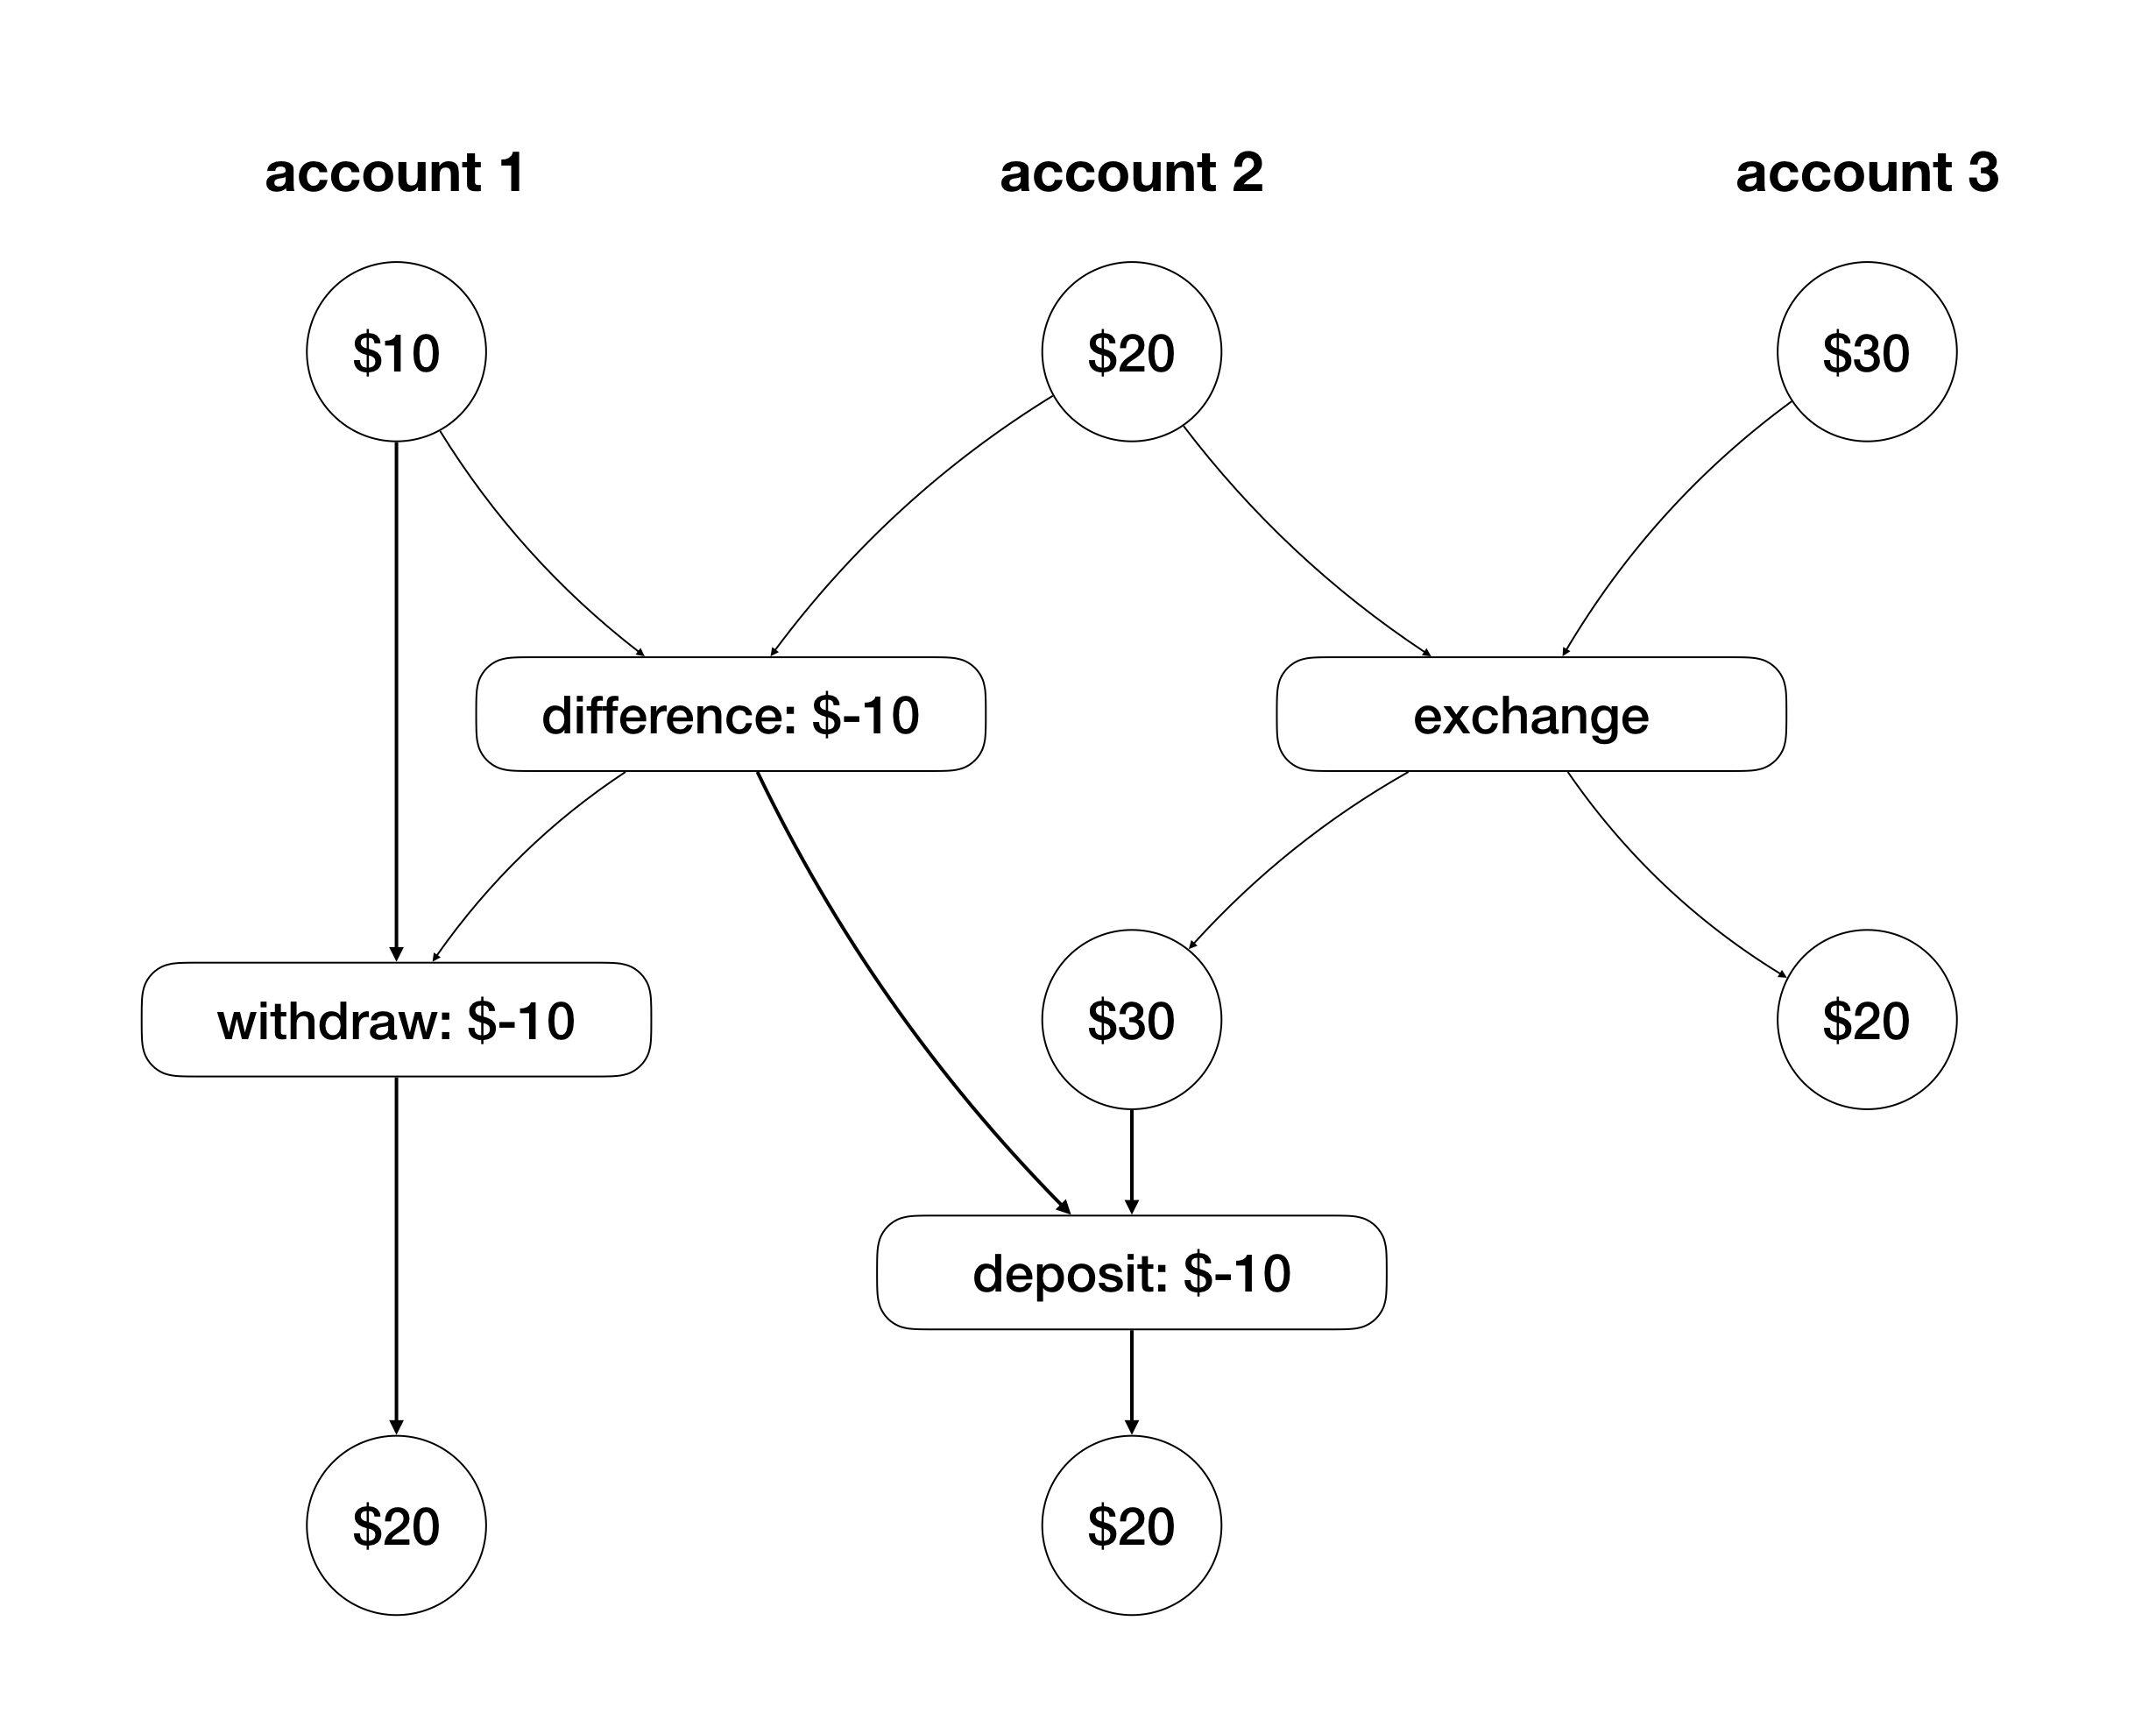
\includegraphics[width=.7\textwidth,height=.7\textheight,keepaspectratio]{1.png}
\end{center}

On the other side, since the \texttt{deposit} procedure and the \texttt{withdraw} procedure are serialized, then deposits and withdrawals cannot be interleaved by other changes. Therefore, due to the first version of the account-exchange program, any difference withdrawn from \texttt{account1} would be deposited into \texttt{account2} with the same amount. Hence, the sum of the balances in the accounts will be preserved after any number of concurrent exchanges.

The following timing diagram shows how even this condition would be violated if we did not serialize the transactions on individual accounts.

\begin{center}
    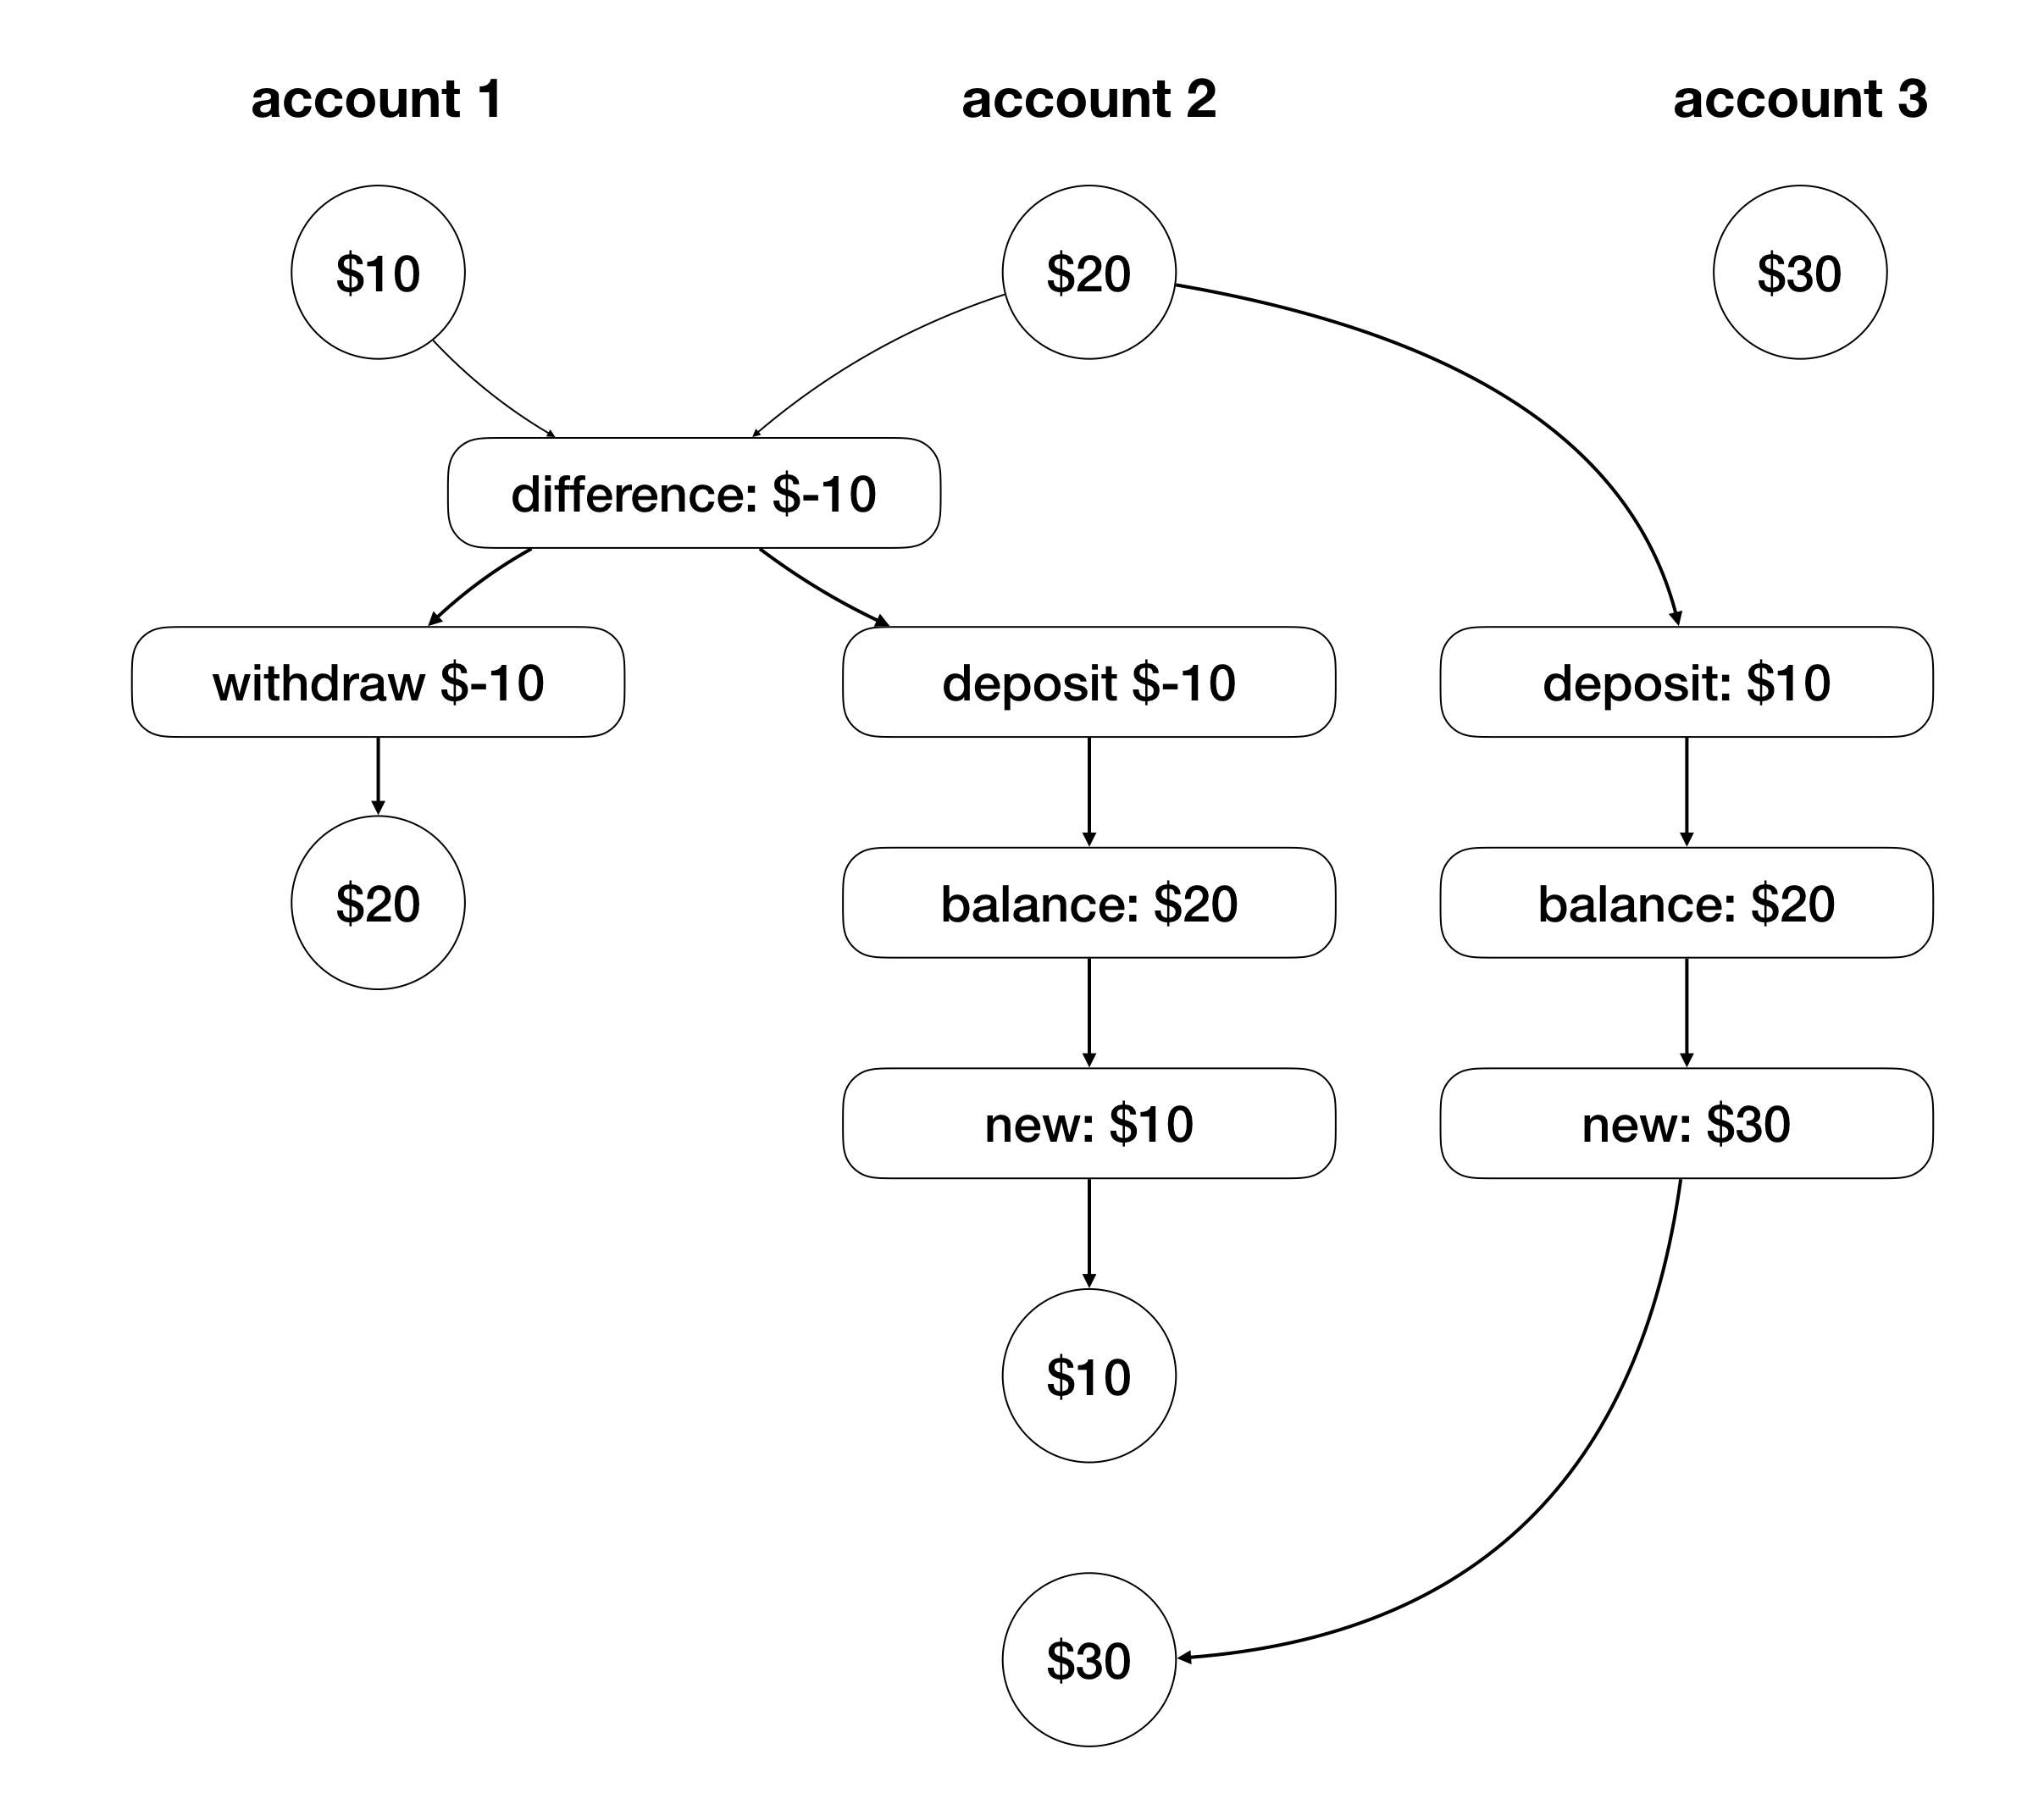
\includegraphics[width=.7\textwidth,height=.7\textheight,keepaspectratio]{2.png}
\end{center}

\end{document}
